\section{Classification of gapped one-dimensional phases}\label{sec:1Dphases}
Recall that in the classical Landau paradigm phases of matter are classified by their symmetry-breaking pattern $G\rightarrow H\subseteq G$~\cite{Landau1937,Chen2025}. Additional phases arise in the quantum mechanical setting since the entanglement degrees of freedom can transform in discrete distinct ways under the residual symmetry group $H$. Concretely, for one-dimensional \emph{bosonic} systems, these classes are organised in the \emph{second cohomology group} of $H$ over $\rU(1)$, denoted by $H^2(H,\rU(1))$ and defined below. Notably, for finite $H$ the second cohomology group $H^2(H,\rU(1))$ is itself finite\footnote{Even though the second cohomology group is also finite for some Lie groups such as $H^2(SO(3),\rU(1))\simeq\mbb Z_2$, this is not generically true, not even for compact groups.}, so that the number of gapped phases with residual $H$ symmetry is also finite. One of the great achievements of tensor networks and in particular MPS, is that this one-dimensional classification can be completely carried out and understood in that framework, also in the fermionic case~\cite{Chen2010,Schuch2011,Bultinck2016}. Let us also note at this point that for one-dimensional bosonic systems, there exist no non-trivial phases without imposing a symmetry. This is different in the fermionic case, due to the existence of a fermionic superselection rule.

\bigskip\noindent This classification rests on two pillars. The first is the fact that MPS provide a \emph{faithful} representation of gapped ground spaces~\cite{Verstraete2006a}; the second is the (symmetric) parent Hamiltonian construction of MPS~\cite{Cirac2020}. Indeed, as argued above, two Hamiltonians $H_1$, $H_2$ with the same symmetry belong to the same phase if and only if there exists a smooth interpolating Hamiltonian path starting in $H_1$ and ending in $H_2$. Assuming an exact MPS representation of the ground space of both Hamiltonians, one can restate this as the search for an interpolating path of the \emph{symmetric parent} Hamiltonians. Equivalently, one can rephrase this problem as the search for a smooth interpolating MPS path.

\bigskip\noindent Let us for a moment assume that the on-site symmetry $G$ is the full symmetry group of the model; we return to the case where $G$ is a subsymmetry below. In that case, the ground state corresponds to a non-injective MPS, $A^i=\bigoplus_{k=1}^r A^i_k$, with each of the blocks generating an injective MPS. In a certain basis, the symmetry acts on the virtual level of the MPS via the \emph{induced} representation
\begin{equation}
	P_g \bigoplus_{k=1}^r \big( U_k(h) \otimes \bar U_k(h) \big), \quad\forall g\in G,
\end{equation}
where $h\equiv h_{g,r_k}$ depends on $g$ and $k$ as specified below. The $\{U_k(h)\}_h$ are unitary matrices acting on the block $k$. The representation $P_g$ permutes the injective blocks, and it is assumed that this permutation acts \emph{transitively}. If we denote by $\pi_g$ the action of $P_g$ on the labels $k$, transitivity means that for every two blocks $k_1$, $k_2$ there exists some $g\in G$ such that $\pi_g(k_1)=k_2$.

We subsequently choose an arbitrary but fixed \emph{reference} block denoted by $k_0$.  This thereby specifies the \emph{stabiliser} subgroup $H\subseteq G$ defined as:
\begin{equation}
	H := \{g\in G \,|\, \pi_g(k_0) = k_0\}.
\end{equation}
Note that choosing a different reference block $k_0'$ would result in a stabiliser group \emph{conjugate}, and thus \emph{isomorphic}, to $H$.

From the \emph{orbit-stabiliser theorem}, combined with transitivity of $P_g$, it follows that the number of blocks is given by $|G/H|$. Let $r_k$, with $k=1,2,\dots,r=|G/H|$, denote a set of representatives of the cosets $G/H$, with $r_{k_0}=\mbb 1$. The group element $h_{g,r_k}\in H$ is then defined via:
\begin{equation}
	gr_k = r_{k'} h_{g,r_k}.
\end{equation}
In fact, it can be shown that the $U_k(h)$'s furnish a \emph{projective} representation of $H$, and the corresponding \emph{topological index} is precisely what encodes the SPT phase of the surviving symmetry. We relegate the discussion of this to the next paragraph.

As anticipated above, $G$ could be a subsymmetry of the full symmetry of the model. In that case, the MPS could exhibit an additional block structure, viz. $A^i = \bigoplus_K\bigoplus_k A_k^i$, signalling the breaking of the larger symmetry. This degeneracy is however not protected by the symmetry $G$, meaning it can be lifted by perturbing the Hamiltonian with symmetric terms. Altogether, this makes precise the above statement that non-injectivity of an MPS is the tensor network manifestation of symmetry-breaking, and clarifies the role of the subgroup $H\subseteq G$.

\bigskip\noindent We are left to explain the distinct ways an injective MPS can transform under a symmetry group, viz.:
\begin{equation}
	U(g)^{\otimes N} |\Psi[A]\ra \simeq |\Psi[A]\ra, \quad \forall g \in G.
\end{equation}
We use here $G$ to denote the symmetry group of the MPS $|\Psi[A]\ra$, but this could be the residual symmetry in the ground state subspace. A direct application of the fundamental theorem \cref{eq:FundTh} reveals that the MPS tensor itself has to transform, for all $g \in G$, according to:
\begin{equation}\label{eq:gMPS}
	\sum_j U(g)_{ij} A^j = e^{i\chi_g} X_gA^iX_g^\dagger
\end{equation}
for unitary gauge matrices $\{X_g\, |\,  g\in G\}$ and complex phases $\{e^{i\chi_g}\, |\, g\in G\}$ that may depend on the group element $g$. We can now act with two distinct group elements $g,h$ on the MPS in two different ways: by acting with $U(gh)$ directly and invoking the fundamental theorem once as in \cref{eq:gMPS} or by sequentially acting with $g$ and $h$ and making use of \cref{eq:gMPS} twice. Equating both yields:
\begin{equation}
	e^{i\chi_{gh}}X_{gh} A^i X_{gh}^\dagger = e^{i(\chi_g+\chi_h)}X_gX_h A^i X_h^\dagger X_g^\dagger,\quad\forall i,g,h.
\end{equation}
Injectivity of the MPS subsequently implies that $\{e^{i\chi_g}\, |\, g\in G\}$ constitutes a one-dimensional representation of $G$, whereas the $X_g$'s form a \emph{projective} representation of $G$, i.e. they multiply according to $X_gX_h = \psi(g,h) X_{gh}$ for $\rU(1)$ phases $\psi(g,h)$. Imposing associativity of the matrix multiplication constrains these phases and shows that they adhere to a consistency condition known as the \emph{2-cocycle condition}:
\begin{equation}\label{eq:2cocycle}
	\psi(g,h)\psi(gh,k) = \psi(g,hk)\psi(h,k), \quad \forall g,h,k\in G.
\end{equation}
Solutions of \cref{eq:2cocycle} form an abelian group $Z^2(G,\rU(1))$ under pointwise multiplication.	 Among these, the trivial solutions, or \emph{coboundaries}, take the form $\psi(g,h)=\frac{\phi_{gh}}{\phi_g \phi_h}$, for any function $\phi:G\rightarrow\rU(1)$. In the jargon of group cohomology such a trivial solution is referred to as a \emph{coboundary} and they constitute a normal subgroup $B^2(G,\rU(1))\trianglelefteq Z^2(G,\rU(1))$. Notably, rescaling of the gauge matrices with arbitrary phases $X_g \mapsto \phi_g X_g$ maps the corresponding 2-cocycle to one differing by the coboundary $\phi_g$, leading to a physical redundancy. Therefore, one \emph{quotients by} such solutions in solving \cref{eq:2cocycle}, leading to equivalence classes of 2-cocycles. Two 2-cocycles $\psi\sim\psi'$ are thus considered cohomologically equivalent if they are related via a coboundary and these equivalence classes form the quotient group $H^2(G,\rU(1)):= Z^2(G,\rU(1))/B^2(G,\rU(1))$ which is the anticipated \emph{second cohomology group} of $G$ over $\rU(1)$.

\bigskip\noindent An MPS that transforms projectively on the virtual level as per \cref{eq:gMPS} is characterised by \emph{symmetry-protected degeneracies} in its entanglement spectrum, as well as the existence of localised \emph{edge modes} on open chains~\cite{Pollmann2009a,Pollmann2009b}. The existence of both follows from the fact that, contrary to linear representations, there exist \emph{no} cohomologically non-trivial \emph{one-dimensional} projective representations. As an illustrative example, consider the $SO(3)$-symmetric ground state of the antiferromagnetic spin 1 Heisenberg model. Since the \emph{projective} representations of $SO(3)$ can be identified with the \emph{half-integer linear} representations of its universal cover, $SU(2)$, the entanglement spectrum of the ground state is organised in multiplets of \emph{even} dimension. This is demonstrated in \cref{fig:HeisenbergEntanglement} where the first 48 Schmidt values of the ground state are plotted.
\begin{figure}[htb]
	\centering
	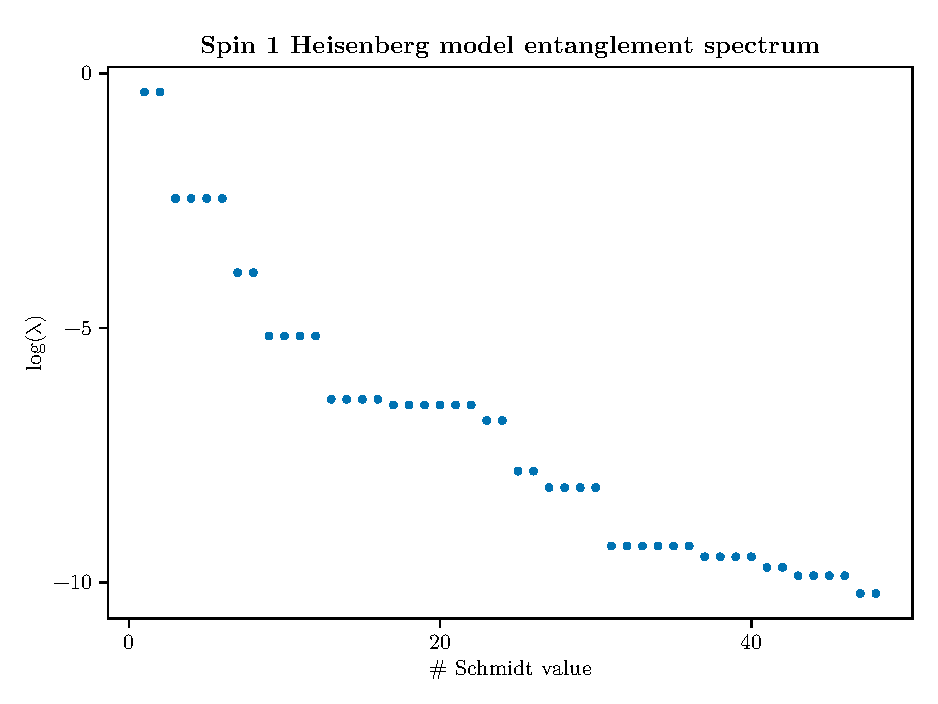
\includegraphics[width=0.7\linewidth]{plots/HeisenbergEntanglementSpectrum.pdf}
	\caption{The entanglement spectrum of the spin 1 Heisenberg model ground state in the thermodynamic limit with bond dimension 48. Created with MPSKit.jl~\cite{VanDamme}.}
	\label{fig:HeisenbergEntanglement}
\end{figure}

As anticipated above, a natural basis for the edge modes is given by the virtual degrees of freedom of the MPS ground state near the boundaries. Indeed, a uniform MPS on open boundary conditions,
\begin{equation}
	\ket{\Psi[A]} = \sum_{\{i_j\}} (A^{i_1}A^{i_2}\cdots A^{i_N})_{\alpha\beta} \ \ket{i_1,i_2,\dots,i_N},
\end{equation}
corresponds to $\chi^2$ states $\ket{\Psi[A], \alpha,\beta}$ that have the same energy for the parent Hamiltonian. Naively, we would thus count $\chi^2$ ground states on the open chain, but some of these modes can be gapped out by turning on additional terms in the Hamiltonian. However, as long as these additional terms respect the symmetry, a certain amount of degeneracy is persistent; these edge modes transform under the symmetry action according to
\begin{equation}
	U(g)^{\otimes N}\ket{\Psi[A],\alpha,\beta} = \sum_{\alpha',\beta'} (X_g)_{\alpha\alpha'} (\bar X_g)_{\beta\beta'}\,\,\ket{\Psi[A],\alpha',\beta'},
\end{equation}
so that at least a two-fold degeneracy persists.

\bigskip\noindent This concludes phase classification in the one-dimensional setting where the symmetry acts via a unitary (tensor product) group representation. To summarise, phases are classified by pairs $(H,[\psi])$ where $H\subseteq G$ is a subgroup up to conjugacy and $[\psi]$ is a class taking values in $H^2(H,\rU(1))$~\cite{Chen2010,Schuch2011}.

Remarkably, these data also classify (indecomposable) \emph{module categories} $\mc R(H,\psi)$ over the \emph{fusion category} $\Vect_G$~\cite{Ostrik2001,Etingof2015}. \emph{Simple objects} of the corresponding module category are labelled by cosets $\{r_1H,r_2H,\dots\}$ and $\mc R(H,\psi)$ carries a natural $\Vect_G$ action induced by $g\act rH:= (gr)H$. This observation suggests the physical interpretation where the gapped ground states are identified with the simple objects, and the action $\act$ with the action of the on-site $G$ symmetry on the ground state subspace. 

This observation is more than a formal analogy and is the first indication of a correspondence between module categories and gapped phases of matter. The \emph{generalised Landau paradigm}, the subject of \cref{sec:GenLandau}, stipulates that this correspondence persists to one-dimensional (lattice) models with a symmetry described by a generic fusion category $\mc C$~\cite{Thorngren2019,GarreRubio2022,Bhardwaj2023,Lootens2024}. More precisely, it states that the different gapped phases are given by the different module categories $\mc P$ over $\mc C$, with the simple objects labelling the ground states and the \emph{module action} describing the symmetry action on them.